\chapter{ทฤษฎีที่เกี่ยวข้อง}
\label{ch:theory}
ในโครงงานศึกษาวิจัยนี้ เป็นการการประยุกต์ใช้เทคนิคการประมวลผลภาพ เพื่อตรวจสอบว่าภาพของแสตมป์สุราเป็นของแสตมป์จริงหรือปลอม ในบทนี้จะพิจารณาหลักทฤษฎีพื้นฐานที่ใช้ในวิธีการประมวลผลภาพ~\cite{Kosin48} ในส่วนของการประมวลผลที่นำมาใช้ในโครงงานศึกษาวิจัยนี้

\section{การแทนภาพดิจิทัลและการแปลงภาพ}
ภาพดิจิทัล (digital image) จะถูกแทนด้วยเมตริกของข้อมูลบ่งบอกสี โดยการใช้หนึ่งตำแหน่งของเมตริกเพื่อแทนข้อมูลจุดหนึ่งของภาพเรียกว่า พิกเซล (pixel)  จำนวนของพิกเซลต่อภาพบ่งบอกถึงความละเอียดของภาพ เช่น ภาพที่ใช้แสดงผลในระบบโทรทัศน์ที่เรียกว่า HD เป็นภาพที่มีขนาดพิกเซลเป็น $1208\times 720$ โดยตัวเลขแรกเป็นจำนวนคอลัมภ์ ซึ่งแปรตรงกับความยาวในแนวนอน

การบอกข้อมูลแสงของแต่ละพิกเซลมีหลายวิธี แต่เราสามารถแบ่งภาพได้เป็น 3 กลุ่มตามลักษณะของข้อมูลแสงคือ ภาพสี (color image) ภาพระดับสีเทา (grayscale image) และภาพขาวดำ (binary image) โดยภาพสีสามารถแปลงไปเป็นภาพระดับสีเทา และภาพระดับสีเทาสามารถแปลงไปเป็นภาพขาวดำได้ 

\subsection{การบอกข้อมูลแสงของภาพสีด้วยระบบสีอาร์จีบี}
ในกรณีของภาพสี แม้ว่าจะมีหลายวิธีที่สามารถบอกข้อมูลสี แต่วิธีที่ได้รับความนิยมสูงสุดในกล้องถ่ายภาพดิจิทัลคือ ระบบสีอาร์จีบี (RGB color system) ทั้งนี้เนื่องจาก โดยตามธรรมชาตินั้น สีแต่ละสีเกิดจากการผสมกันของเซตของแม่สี และแม่สีที่ได้รับความนิยมสูงสุดคือ สีแดง (Red) สีเขียว (Green) และสีน้ำเงิน (Blue) จึงเรียกระบบการบอกสีด้วยแม่สี 3 ตัวนี้ว่าระบบสี RGB  

ภายใต้ระบบสีอาร์จีบี โดยทั่วไปจะใช้ข้อมูล 8 บิต หรือ 256 ระดับเพื่อบอกระดับแสงของแต่ละแสง  ดังนั้นแต่ละพิกเซลจะต้องใช้ข้อมูลขนาด 24 บิต เพี่อบ่งบอกว่าเป็นสีอะไร  กล่าวได้ว่าในระบบสีอาร์จีบี 24 บิทเช่นนี้จะมีสีที่แตกต่างกันได้ทั้งหมด เท่ากับ 16,777,216 สี คำนวณจากแต่ละสีมี 256 ระดับ ( $2^{8}$) จำนวนระดับที่แตกต่างกันทั้งหมดจึงเป็น $256\times 256\times 256 = 16,777,216$  เราเรียกจำนวนสีทั้งหมดของระบบสีว่าเป็น ปริภูมิสี (Color Space) ซึ่งในกรณีของระบบสีอาร์จี  ปริภูมิสี (Color Space) จะมีลักษณะเป็นแบบลูกบาศก์ดังแสดงในรูปที่~\ref{fig:2-1} 

\vspace{1em}
\begin{figure}[!ht]
\centering
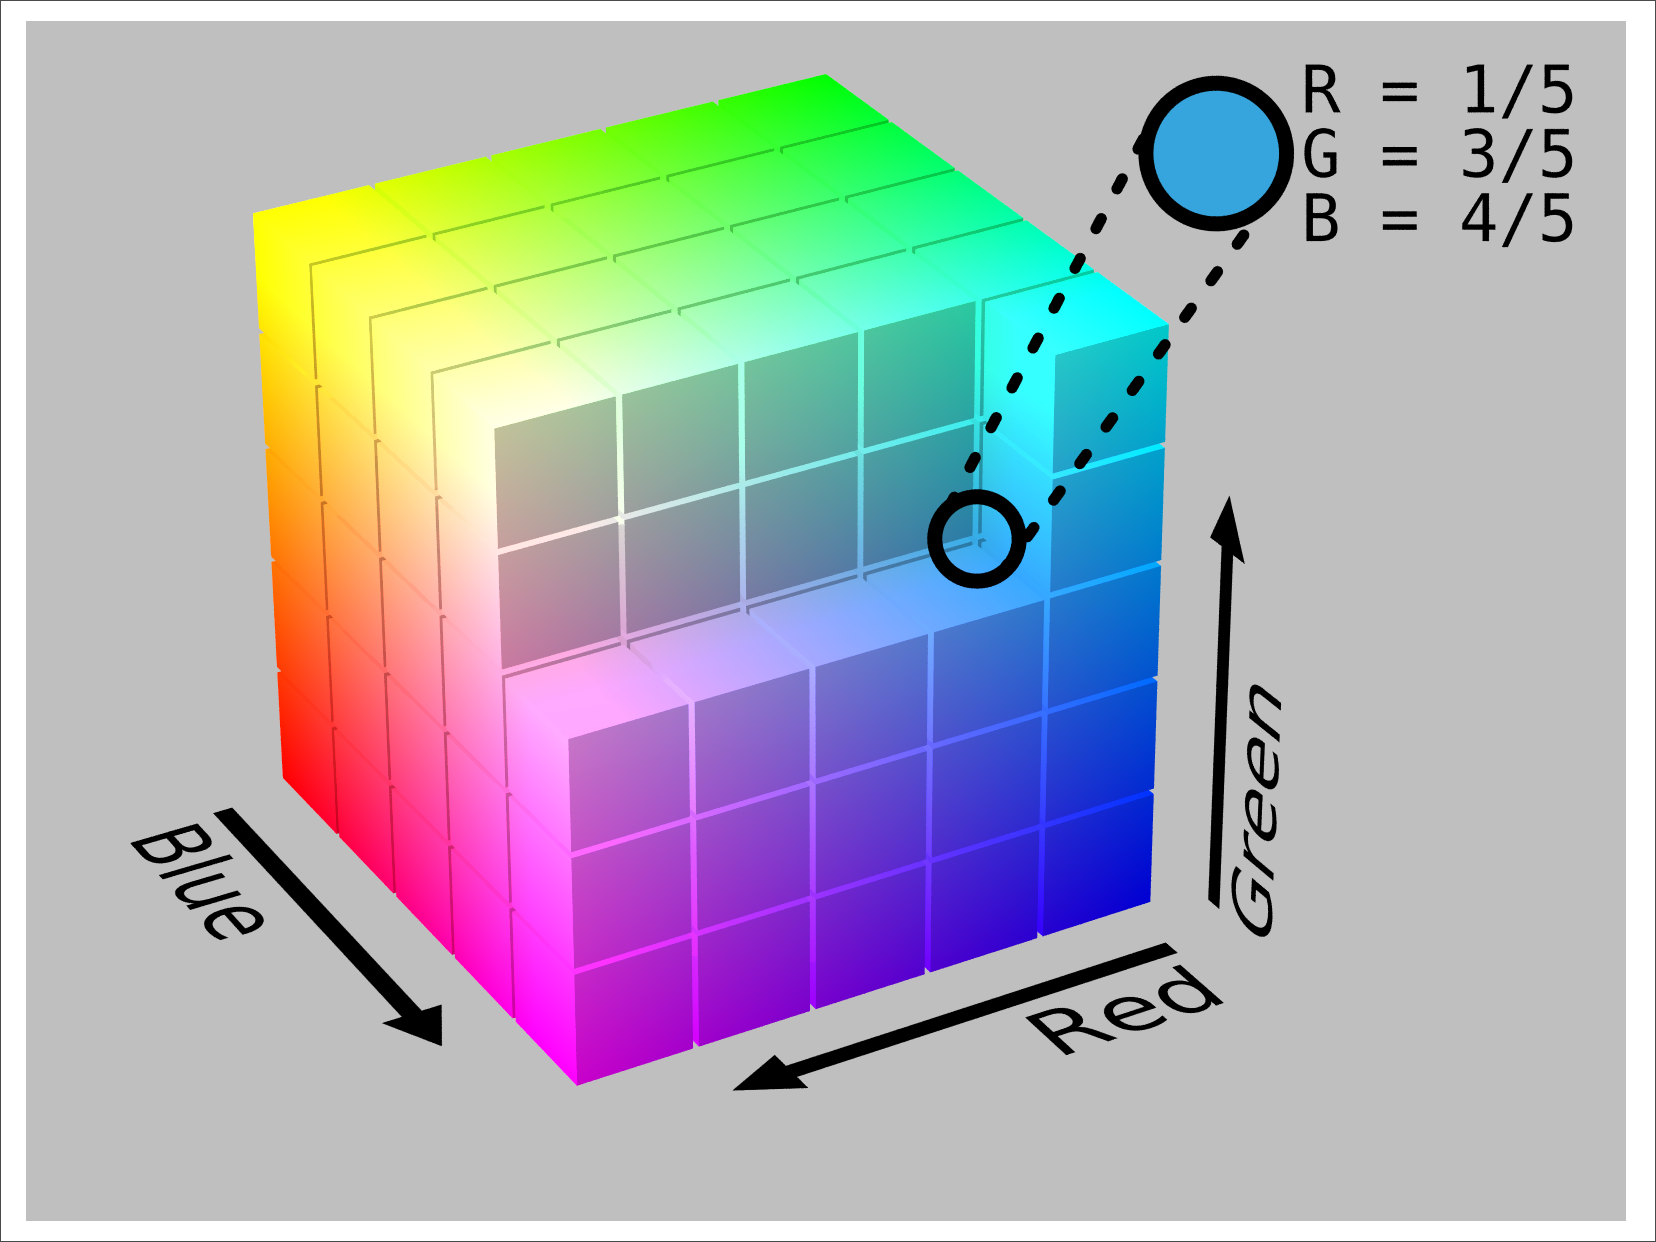
\includegraphics[width=0.9\textwidth]{rgb-cube}
\caption{ปริภูมิสี (Color Space) ในแบบลูกบาศก์ของพิกัดสีอาร์จีบี~\cite{RGBspace}}
%(ที่มา: http://wcm-birding.blogspot.com/2016/, 2560)
\label{fig:2-1}
\end{figure}

\begin{figure}[!ht]
\centering
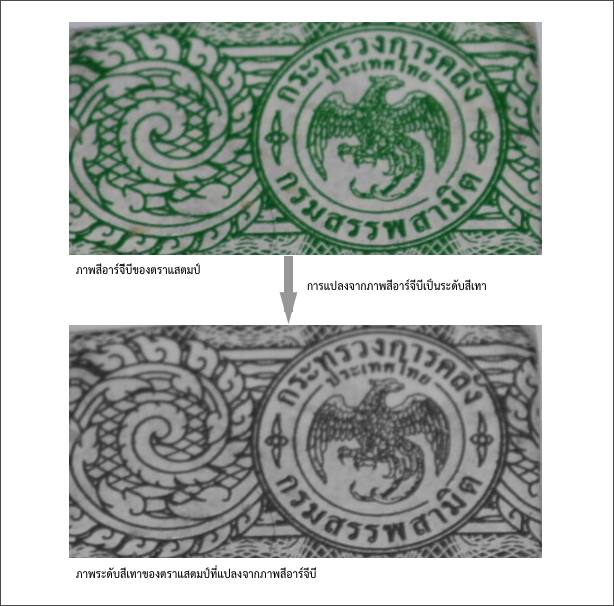
\includegraphics[width=0.9\textwidth]{rgb2gray-example}
\caption{ภาพระดับสีเทาที่ได้จากการแปลงจากภาพสีอาร์จีบี}
%(ที่มา: บริษัท เจ.เอฟ.แอดวาน.เมด.จำกัด, 2560)
\label{fig:rgb2gray}
\end{figure}

\subsection{ภาพระดับสีเทา}
ข้อมูลแสงในแต่ละพิกเซลของภาพระดับสีเทาเป็นค่าความเข้มแสง (light intensity) ระดับความเข้มแสงแต่ละระดับแสดงผลออกมาเป็นสีเทาหนึ่งสี  โดยระดับความเข้มสูงสุดจะเป็นสีขาว และระดับความเข้ม 0 จะเป็นสีดำ  จำนวนระดับสีเทา  (grayscale) ขึ้นอยู่กับจำนวนบิตของการบอกระดับ เช่นภาพระดับสีเทาขนาด 8 บิต บอกระดับสีเทาได้ 256 ระดับจาก 0 ถึง 255 

เราสามารถคำนวณระดับสีเทาของสีอาร์จีบีได้โดยการหาค่าเฉลี่ยแบบมีน้ำหนัก (weighted average) ของระดับแสงของแม่สี RGB เนื่องจากโดยธรรมชาติแล้วการมองเห็นแสงแต่ละสีไม่เท่ากัน   ค่าน้ำหนักที่เป็นที่นิยมในการคำนวณเพื่อแปลงสีอาร์จีบีเป็นระดับสีเทาเป็นไปตามสมการที่~\ref{eq:rgb2grey}  

\begin{equation}
Grey = 0.299R + 0.587G + 0.114 B \label{eq:rgb2grey}
\end{equation}
เมื่อ $R$, $G$ และ $B$ เป็นระดับแสงสีแดง สีเขียว และสีน้ำเงินตามลำดับ 
รูปที่~\ref{fig:rgb2gray} แสดงภาพสีเทาที่ได้จากการแปลงภาพสีอาร์จีบี


\subsection{ภาพขาวดำ (Binary Image) และการแปลงภาพระดับสีเทาเป็นภาพขาวดำ}
ข้อมูลแสงในแต่ละพิกเซลของภาพขาวดำ (Binary image) มีเพียง 2 สถานะ ซึ่งสามารถแทนด้วยข้อมูล 1 บิต โดย 0 แทนสีขาว และ    1 แทนสีดำ  เราอาจพูดได้ว่าภาพขาวดำก็คือภาพระดับสีเทาที่บอกระดับแสงด้วยข้อมูล 1 บิต 

กระบวนการในการแปลงภาพระดับสีเทาเป็นภาพขาวดำ เป็นการกระทำพื้นฐาน (basic operation) ของการประมวลผลภาพ  โดยมีหลายวิธีการแปลงภาพระดับสีเทาเป็นภาพขาวดำ เช่น วิธีการหาขอบ (edge detection) แต่ไม่ว่าจะเป็นวิธีการแปลงใดก็ตาม หลักการของการแปลงภาพระดับสีเทาเป็นภาพขาวดำคือการเปรียบเทียบกับค่าเทรซโฮลด์ตามสมการที่~(\ref{eq:background-thresholding})

\begin{equation}
B(x,y) = \left\{ \begin{array}{ll}
1, \mbox{ถ้าเงื่อนของการแปลงเป็นจริง เช่น}\ I(x,y) >= I_{th}\\
0, \mbox{กรณีอื่น ๆ}
\end{array}\right. \label{eq:background-thresholding}
\end{equation}
เมื่อ $0$ แทนส่วนสีดำ, $1$ แทนส่วนสีขาว, $B(x,y)$ และ $I(x,y)$ เป็นค่าข้อมูลสีของพิกเซล $(x,y)$ ในภาพขาวดำและภาพระดับสีเทา ตามลำดับ และในกรณีตัวอย่างนี้ $I_{th}$ เป็นค่าระดับเทรซโฮลที่ใช้


เงื่อนไขในการแปลจุดพิกเซลของภาพให้เป็นสีขาว ($1$)  หรือสีดำ ($0$)  นั้นขึ้นอยู่กับจุดประสงค์ของการแปลงภาพ ยกตัวอย่างวิธีการแปลงเป็นภาพขาวดำง่ายที่สุดคือ การใช้ระดับความเข้มแสงเป็นเทรซโฮลด์ในการแยกเพื่อแยกภาพออกเป็น 2 ลักษณะพื้นที่  ในบางกรณี เงื่อนไขการแบ่งจะขึ้นอยู่กับข้อมูลสีของพื้นที่รอบจุดพิกเซลที่สนใจ

%ที่นำมาใช้ ในกรณีของการลบภาพพื้นหลัง  มีจุดประสงค์ของการแยกระหว่างภาพพื้นหลัง (background) ออกจากภาพส่วนหน้า (foreground) ซึ่งเป็นส่วนที่สนใจในการนำไปประมวลผล การลบพื้นหลังใช้หลักการของการหาฮิสโตแกรม (histogram)  ของภาพซึ่งเป็นการนับการกระจายความเข้มแสงภายในภาพว่าอยู่ที่ส่วนใด ตามธรรมชาติของภาพแล้ว พื้นหลังของภาพจะมีความเข้มที่จับกลุ่มกันอยู่ทางด้านใดด้าหนึ่ง กล่าวคือสำหรับภาพที่พื้นหลังค่อนไปทางมืด ความเข้มของภาพพื้นหลังจะรวมกลุ่มอยู่ทางด้านซ้ายของฮิสโตแกรม แต่กลับกันภาพพื้นหลังมีความสว่าง เช่นภาพถ่ายของหิมะที่ปกคลุมพื้นที่ จะมีความเข้มของภาพพื้นหลังที่จับกลุ่มกันอยู่ทางด้านขวาของฮิสโตแกรม ดังแสดงในรูปที่~\ref{fig:bw}

จะเห็นว่าวิธีการเทรซโฮลเป็นวิธีการแบ่งพื้นที่ในภาพตามช่วงของระดับความเข้มแสง ซึ่งหลักการนี้สามารถใช้ได้กับข้อมูลระดับความเข้มแสงได้ทุกชนิด เช่น เราสามารถแบ่งภาพเป็น 2  ส่วนตามระดับสีเขียว หรือสีแดง หรือสีน้ำเงิน สีใดสีหนึ่งเพียงสีเดียวก็ได้ ด้วยหลักการเดียวกัน เราสามารถการแบ่งพื้นที่ของภาพออกเป็นมากกว่า 2 ส่วนก็ได้ เช่น เราอาจต้องการแบ่งพื้นที่ในภาพเป็น 4 ส่วน ซึ่งแทนด้วยข้อมูล 2 บิต ซึ่งในกรณีนี้จะต้องมีค่าเทรซโฮล 2 ตัวเพื่อการแบ่งระดับความเข้มแสงเป็น 4 ส่วน เรียกวิธีการแบ่งระดับที่ผลลัพธ์มีมากกว่า 2 ส่วนว่า การแบ่งหลายส่วน (multiband threshold)


\section{การหาขอบของวัตถุ (Edge Detection)}
การหาขอบ (Edge Dectection) ภายในภาพ เป็นการกระทำพื้นฐาน (basic operation) ของการประมวลผลภาพ  ที่มีการนำไปใช้จำนวนมาก เนื่องจากขอบภาพเป็นสารสนเทศพื้นฐานที่สำคัญ กล่าวคือขอบภายในภาพเป็นสารสนเทศพื้นฐานในการแบ่งส่วน การบอกรูปร่าง ซึ่งจะนำไปสู่การตรวจจับหาส่วนของภาพที่สนใจ (interested region) ทำให้เกิดตัดข้อมูลภาพส่วนที่ไม่เกี่ยวข้องออกไป เช่น ในโครงงานศึกษาวิจัยนี้ ต้องการตัดเอาเฉพาะส่วนที่เป็นตราของแสตมป์เท่านั้น


การหาขอบเป็นการแปลงภาพระดับสีเทาเป็นภาพขาวดำอย่างหนึ่ง โดยต้องการให้ส่วนที่เป็นสีขาวแทนขอบของวัตถุที่อยู่ในภาพ เทคนิคของการหาขอบมีหลายวิธี  แต่สามารถแบ่งออกได้เป็น 2 กลุ่ม หลักคือ วิธีการเกรย์เดียน (Gradient method) และ วิธีการลาปาซ (Laplacian method) สำหรับการหากรอบด้วยวิธีเกรย์เดียน  จะใช้การหาจุดต่ำสุดและจุดสูงสุดในรูปของอนุพันธ์อันดับหนึ่งของภาพ  วิธีการหาขอบในกลุ่มนี้ได้แก่ Sobel, Roberts, Prewitt และ Canny เป็นต้น ส่วนวิธีลาปาซ  จะหาขอบโดยใช้อนุพันธ์อันดับ 2 โดยใช้จุดที่ค่าจุดศูนย์ (Zero-crossing) ของอนุพันธ์อันดับ 2 ในภาพ ตัวอย่างวิธีการหาขอบในกลุ่มนี้ได้แก่ Laplacian of Gussian และ Marrs-Hildreth สำหรับโครงงานศึกษาวิจัยนี้ได้เลือกใช้วิธี Canny ในการหาขอบภาพ เพราะจากเอกลักษณ์ของภาพ  คือ  มีรูปร่างที่เด่นชัด ทำให้ไม่จำเป็นที่การหาขอบภาพจะต้องละเอียดมาก  แต่จะต้องสามารถหาขอบภาพได้ผลลัพธ์ในระดับ  ดังนั้นจึงเลือกใช้วิธี Canny 

การหาขอบด้วยวิธี Canny ใช้วิธีเกรย์เดียน ซึ่งมีขั้นตอนดังนี้
\begin{enumerate}
\item กรองภาพด้วยการกรอง Gaussian
\item หาเวคเตอร์เกรย์เดียนของพิกเซล ($x,y$) ตามสมการที่~(\ref{eq:gradient})
\begin{equation}
\nabla f(x,y) = \left[
\begin{array}{l}
G_x(x,y)\\
G_y(x,y)
\end{array}
\right] = \left[
\begin{array}{l}
\frac{\partial }{\partial x}f(x,y)\\
\frac{\partial }{\partial y}f(x,y)
\end{array}
\right]\label{eq:gradient}
\end{equation}
เมื่อ $\nabla f(x,y)$ เป็นเวคเตอร์เกรย์เดียนที่พิกเซล $(x,y)$ ของอนุพันธ์ย่อยของความเข้มแสง $f(x,y)$  ในแกน $x$ และแกน $y$ โดย $G_x$ และ $G_y$ เป็นอนุย่อยของ $f(x,y)$ ในแนวแกน $x$ และ $y$ ตามลำดับ
\item เปรียบเทียบขนาดของเกรย์เดียน $\nabla f(x,y)$  ตามสมการที่~(\ref{eq:gradient-abs}) กับค่าเทรซโฮลด์ $T$  เพื่อตัดสินว่าพิกเซล $(x,y)$ เป็นส่วนหนึ่งของขอบหรือไม่ตามสมการที่~(\ref{eq:edge}) และหาว่าขอบที่จุดพิกเซล $(x,y)$ อยู่ในทิศทาง $0$, $45$, $90$, หรือ $135$ องศา จากการหามุม $\theta (x,y)$ ตามสมการ~\ref{eq:gradient-theta}
\begin{eqnarray}
G(x,y) &=& |\nabla f(x,y)| \sqrt{G_x(x,y)^2 + G_y(x,y)^2}\label{eq:gradient-abs}\\
\theta (x,y) &=& \tan^{-1}\frac{G_y}{G_x}\label{eq:gradient-theta}\\
E(x,y) &=&\left\{ \begin{array}{ll}
1 & \mbox{if}\ G(x,y)  > T\\
0 & \mbox{otherwise}
\end{array}
\right.\label{eq:edge}
\end{eqnarray}
\item ขจัดขอบปลอมโดยวิธี non-maximum suppression
\item ใช้เทคนิคของ 2 เทรซโฮลด์ (Double threshold) ในการกำจัดขอบปลอม
\item ต่อขอบ (edge tracking) ด้วยเทคนิคฮิสเตอรีซีส (hysteresis)
\end{enumerate}

\begin{figure}[!ht]
\centering
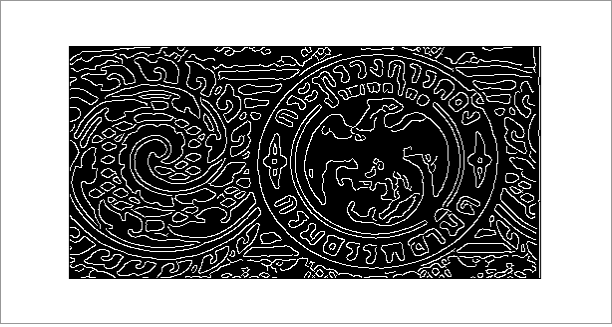
\includegraphics[width=0.9\textwidth]{edge-example}
\caption{ตัวอย่างของผลการหาขอบด้วยวิธี Canny ของภาพระดับสีเทาในรูปที่~\ref{fig:rgb2gray}}
%(ที่มา: บริษัท เจ.เอฟ.แอดวาน.เมด.จำกัด, 2560)
\label{fig:edege-example}
\end{figure}

รูปที่~\ref{fig:edege-example} แสดงภาพผลลัพธ์ของการหาขอบด้วยวิธี Canny ของภาพแสตมป์ในรูปที่~\ref{fig:rgb2gray} 

\section{การแปลงฮัฟวงกลม (Circle Hough Transform)}
การแปลงฮัฟ (Hough transform) เป็นเทคนิคสำหรับการตรวจจับส่วนของเส้นตรง (line) หรือเส้นโค้ง (curve) ภายในภาพ แม้ว่าโดยหลักการแล้ววิธีการแปลงฮัฟจะสามารถใช้กับภาพอินพุทที่เป็นภาพระดับสีเทาก็ได้ แต่เราจะใช้การแปลงฮัฟกับภาพขาวดำ หรือภาพที่เป็นผลจากการหาขอบ เพราะวิธีการแปลงฮัฟต้องใช้การคำนวณและหน่วยความจำสูง

\begin{figure}[!ht]
\centering
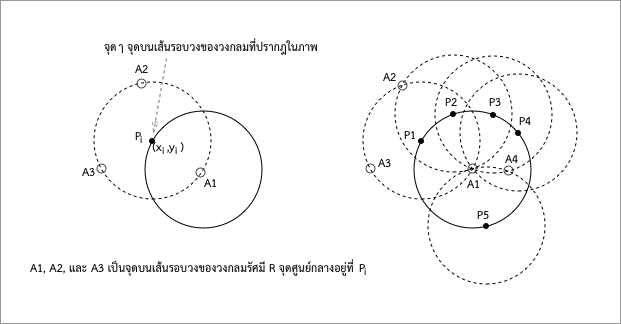
\includegraphics[width=0.9\textwidth]{Hough-transform-concept}
\caption{แนวคิดของการแปลงฮัฟวงกลม (Circle Hough Transform)}
%(ที่มา: บริษัท เจ.เอฟ.แอดวาน.เมด.จำกัด, 2560)
\label{fig:hough-concept}
\end{figure}
การแปลงฮัฟวงกลม เป็นกรณีพิเศษของการแปลงฮัฟ โดยมีหลักการว่า ถ้าเราสร้างวงกลมรอบจุดที่อยู่บนเส้นรอบวงของวงกลม วงกลมเหล่านี้จะไปตัดกันที่จุดศูนย์กลางของวงกลม ตามที่แสดงในรูปที่~\ref{fig:hough-concept} ด้านขวาจะเห็นว่า  วงกลมรัศมี $R$ 5 วงที่มีจุดศูนย์กลางที่จุด $P_1$, $P_2$, $P_3$, $P_4$, และ $P_5$ ซึ่งต่างเป็นเป็นจุดบนเส้นรอบวงของวงกลมรัศมี $R$ ในภาพขาวดำ จะตัดกันที่จุด $A_1$ ซึ่งเป็นจุดศูนย์กลางของวงกลมในภาพขาวดำ 

การแปลงฮัฟวงกลมใช้หลักการดังกล่าว ในการค้นหาจุดศูนย์กลางของวงกลมรัศมี $R$ ดังนี้
สำหรับจุด $P_i = (x_i, y_i)$ ใด ๆ ที่เป็นจุดที่อยู่บนขอบภายในภาพ ในขั้นตอนแรกของการแปลงฮัฟวงกลมจะเป็นการสร้างวงกลมรอบจุด $P_i$ ทุกจุดตามสมการที่~(\ref{eq:circle})
\begin{equation}
(x - x_i)^2 + (y-y_i)^2 = R^2\label{eq:circle}
\end{equation}
โดยที่ $(x_i, y_i)$ เป็นจุดที่อยู่บนขอบ (ค่าความเข้มแสงของจุดเท่ากับ $1$) ในภาพขาวดำที่ได้จากการหาขอบ และ $(x,y)$ เป็นจุดบนวงกลมรัศมี $R$ ที่มีจุดศูนย์กลางงอยู่ที่ $(x_i,y_i)$ ตามที่แสดงในรูปที่~\ref{fig:hough-concept} ด้านซ้ายมือ

ในกระบวนสร้างวงกลมตามสมการ~(\ref{eq:circle}) นั้น จะมีการนับความถี่ของการที่จุด $(x, y)$ ใด ๆ  ไปอยู่บนเส้นรอบวงของวงกลมที่สร้างตามสมการที่~(\ref{eq:circle}) ยกตัวอย่างเช่น ในรูปที่~\ref{fig:hough-concept} ด้านขวามือมีการสร้างวงกลม 5 วง จุด $A_3$ เป็นจุดที่อยู่บนเส้นรอบวงของวงกลมเหล่านี้ 1 ครั้ง ในขณะที่จุด $A_2$ และ $A_4$ เป็นจุดที่อยู่บนเส้นรอบวงของวงกลม 2 ครั้ง และจุด $A_1$ อยู่บนเส้นรอบวงของวงกลม 5 วง  ผลลัพธ์ของการกระทำดังกล่าวนี้จะเป็นเมตริกความถี่ของการเกิด โดยที่เมตริกนี้มีค่าที่ตำแหน่ง $(x,y)$ เป็นจำนวนครั้งที่วงกลมตามสมการที่~(\ref{eq:circle}) ไปตัดกันที่จุด $(x,y)$ 

ขั้นตอนต่อมาของการแปลงฮัฟวงกลม เป็นการเลือกจากเมตริกซ์ของจำนวนครั้งที่วงกลมไปตัดกันที่จุด $(x,y)$ ว่าจะจุดใดบ้างที่เป็นจุดศูนย์กลางของวงกลมรัศมี $R$ โดยเกณฑ์ในการเลือกจะมาจาก 2 วิธี คือ (1) การเรียงลำดับ และ (2) การใช้เทรซโฮลด์ หรือทั้ง 2 อย่างรวมกัน วิธีการเรียงลำดับจะใช้ได้กับภาพที่รู้ว่ามีจำนวนของวงกลมรัศมี R อยู่เท่าไร ถ้าทราบจำนวนดังกล่าว สมมุติว่าเป็น $n$ ตัวแล้ว เราสามารถเลือกจุดที่เป็นจุดศูนย์กลางของวงกลม จากการเรียงลำดับแล้วเลือก $n$ ตัวแรก แต่ในกรณีที่ไม่ทราบว่ามีวงกลมอยู่กี่วง การใช้เทรซโอลจะเหมาะสมกว่า กล่าวคือ ถ้าจำนวนความถี่น้อยกว่าค่าเทรซโฮลด์แสดงว่าไม่มีวงกลม แต่ถ้ามากกว่าแสดงว่ามีวงกลม หรือส่วนของวงกลมรัศมี R อยู่

\begin{figure}[!ht]
\centering
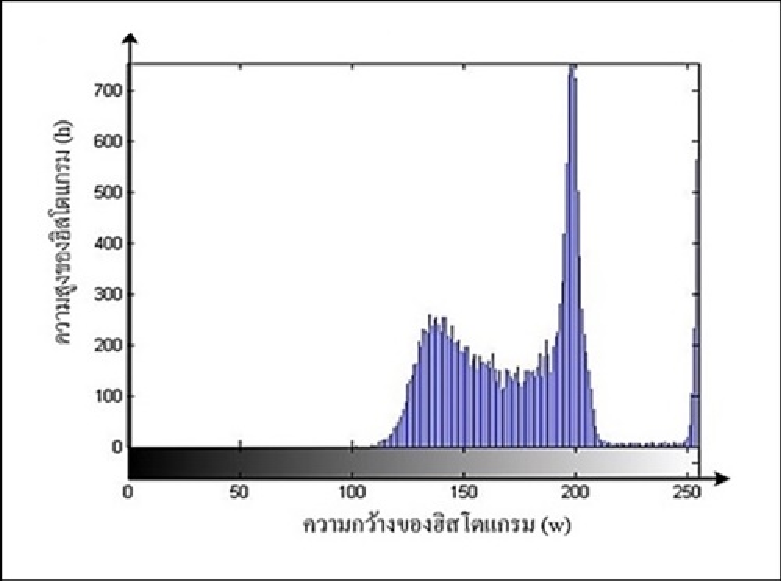
\includegraphics[width=0.9\textwidth]{histogram-example}
\caption{ตัวอย่างฮิสโตแกรมของระดับสีเทาของภาพในรูปที่~\ref{fig:rgb2gray}}
%(ที่มา: บริษัท เจ.เอฟ.แอดวาน.เมด.จำกัด, 2560)
\label{fig:histogram}
\end{figure}

\section{ฮิสโตแกรมของภาพ (Image Histogram)}
ฮิสโตแกรมเป็นการนับจำนวนความถี่ของการเกิดขึ้นของค่าของตัวแปรสุ่มจากกลุ่มข้อมูลจำนวนหนึ่ง ในกรณีของฮิสโตแกรมของภาพขนาด $c\times r$ พิกเซล ตัวแปรสุ่มคือระดับสี หรือระดับความเข้มแสง ซึ่งอาจจะเป็นระดับสีเทา หรือระดับสีใดสีหนึ่งของอาร์จีบี หรือระดับ H ในระบบสี HSV เป็นต้น ส่วนข้อมูลที่ใช้ในการนับคือระดับสีจากทุกพิกเซลของภาพ

ในกระบวนการนับจะต้องมีการสร้างกล่อง (Bin) ที่จะนับข้อมุลลงไป หนึ่งกล่องจะเป็นหนึ่งช่วงของตัวแปรสุ่ม โดยทั่วไปแล้วช่วงทั้งหมดของตัวแปรสุ่มจะแบ่งถูกแบ่งเป็น $n$ กล่องเท่ากัน ในกรณีของภาพ ตัวแปรสุ่มคือระดับความเข้มแสงซึ่งเป็นเลขจำนวนเต็มในช่วง 0 ถึง 255  (ในกรณีของระดับสีขนาด 8 บิท) ดังนั้นการแบ่งที่มีขนาดกล่องเล็กที่สุดคือ การใช้หนึ่งระดับสีเป็นหนึ่งกล่องรวมทั้งหมด  256 กล่อง

ในการสร้างฮิสโตแกรมของภาพ พิกเซลจะถูกตรวจสอบทีละพิกเซลว่ามีค่าระดับสีอยู่ในกล่องใด ผลลัพธ์การพล็อตฮิสโตแกรมจะเป็นการกระจายของโอกาสการเกิด รูปที่~\ref{fig:histogram} แสดงผลของฮสโตแกรมของภาพระดับสีเทาในรูปที่~\ref{fig:rgb2gray}

%
% การสร้าง accumulator cell ในกรณีวงกลมจะเป็น A(i, j) 3 มิติซึ่งพารามิเตอร์จะประกอบด้วย Cx, Cy และ r สำหรับวิธีการคำนวณหาพิกัด x, y ที่อยู่บนวงกลมหรือส่วนโค้งอันเดียวกันจะใช้วิธีการเช่นเดียวกันกับกรณีของเส้นตรง ในทำนองเดียวกันการหาส่วนโค้งและวงกลมด้วย Hough Circle Transform จะใช้สมการ
%
% \begin{displaymath}
%(x-c_x)^{2}+ (y-c_y)^{2}=r^{2}
%\end{displaymath}


